% Chapter 1

\chapter{Introduction}
\label{Chapter1}

\section{Binary black-hole mergers}

At the time of writing the 
% Laser Interferometer Gravitational-Wave Observatory 
LIGO~\cite{LIGOScientific:2014pky} and Virgo~\cite{VIRGO:2014yos} detectors have completed three observing runs, accumulating 90 gravitational-wave (GW) signal candidates with probability of astrophysical origin $> 0.5$~\cite{LIGOScientific:2018mvr, LIGOScientific:2020ibl, LIGOScientific:2021usb, LIGOScientific:2021djp}.
The signals originate from the mergers of compact objects. 
The majority of these are binary black holes (BBHs), and these are the systems of interest throughout this thesis.  
Signals have also been observed from at least one binary neutron star system (GW170817~\cite{LIGOScientific:2017vwq} remains the only unambiguous candidate) and from neutron-star -- black-hole (BH) systems (the most confident candidate being GW200115\_042309~\cite{LIGOScientific:2021qlt}).
GW150914~\cite{LIGOScientific:2016aoc} marked the first direct observation of GWs, as well as the first observation of a BBH merger.
It also marked what can be described in simple terms as the first measurement of a ringing BH.

A prediction of general relativity (GR), GWs are produced by accelerating masses; they are transverse waves which act to expand and contract space.
They can be measured via their influence on freely-falling test masses, which will move relative to each other as space is perturbed.
This is somewhat analogous %~\cite{Saulson:1997ck} 
to the expansion of the Universe, which causes distant galaxies (the test masses) to appear to recede from us due to the expansion of space.
The LIGO and Virgo GW detectors employ interferometry to measure the motion of test masses to extreme precision.
In this setup the mirrors at the end of the interferometer arms act as the freely-falling masses (they are hung as pendulums to isolate them from the environment), and changes in their position can be determined via the light travel time of the interferometer laser.
The detector output is a timeseries of a dimensionless scalar quantity called the strain, $h$, which quantifies the change in position of the mirrors (which can also be thought of as changes to the interferometer arm lengths).

It is understood how the dynamics of compact-object mergers translate to the measured strain, which allows us to learn about the signal origin.
The GW signal from a BBH merger can be split into three stages: the inspiral, merger, and ringdown.
The inspiral corresponds to the two BHs in the binary orbiting each other. 
Unlike in the Newtonian case, the generation of GWs causes the system to lose energy and for the orbit to shrink and spiral. 
This stage in the binary evolution, where the motion of the orbit is slow compared to the speed of light, can be modelled with corrections to the Newtonian case in a post-Newtonian framework~\cite{Blanchet:2013haa}. 
Eventually, the BHs come together in the highly energetic and dynamical merger; this process requires the full nonlinear equations of GR, and is the subject of numerical relativity (NR)~\cite{Duez:2018jaf}. 
Immediately after merging, the final BH is highly distorted. 
As it equilibrates it produces GWs which roughly take the form of a damped sinusoid. 
This is analogous to the ringing a bell makes after it has been struck, and this final stage is called the ringdown.
Just as the early inspiral can be studied by considering deviations to a Newtonian system, the ringdown can be studied by considering perturbations to a static BH spacetime~\cite{Sasaki:2003xr, Pound:2021qin}. 
It is not known beforehand when this perturbative treatment of the final BH becomes valid (i.e., when the ringdown actually starts), and so care must be taken; this will be a recurring theme throughout this work.

\begin{figure}[t]
	\centering
	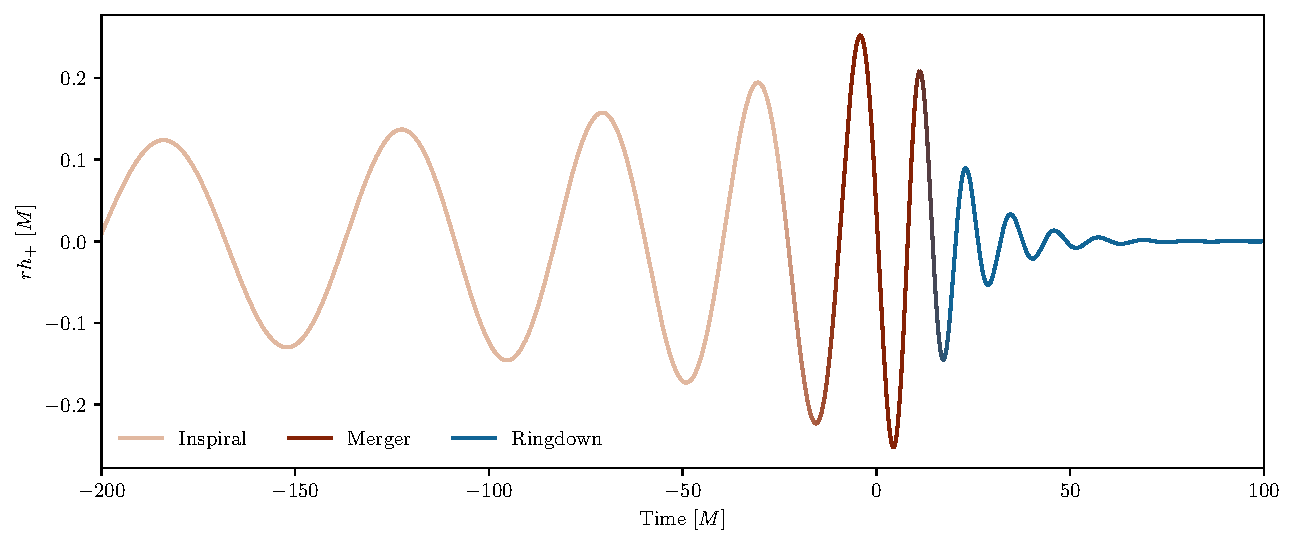
\includegraphics[width=\columnwidth]{Introduction/td_waveform.pdf}
	\caption[The time-domain gravitational-wave signal from a binary black-hole merger]{ 
		The gravitational-wave signal from a binary black-hole merger. This waveform was generated using the NRSur7dq4 surrogate, and projected onto the Hanford detector using parameters consistent with GW150914.}
	\label{fig:ch1:td_waveform}
\end{figure}

The GW signal from these three stages is shown in Fig.~\ref{fig:ch1:td_waveform}.
Plotted is the (noiseless) GW signal projected onto the LIGO Hanford detector, $h$, multiplied by the distance to the source, $r$, as a function of time. 
We use geometric units ($G = c = 1$) to express these quantities in units of the total binary mass, $M$. 
In geometric units we can convert between lengths, masses, and times with appropriate combinations of $G$ and $c$; this means $\mathrm{time}/M$ and $rh/M$ can be made dimensionless quantities. 
Say we had a system with total mass $M = 72\, M_\odot \approx 1.43 \times 10^{32}\,$kg at a distance $r = 440\,$Mpc $\approx 1.36 \times 10^{25}\,$m (chosen because these are consistent with the system properties of the first GW event, GW150914). 
Expressing $M$ in seconds gives us the conversion factor for time:
\begin{equation}
    M \times \frac{G}{c^3} \approx 1.43 \times 10^{32}\, \mathrm{kg} \times \frac{6.67 \times 10^{-11}\, \mathrm{m}^3\, \mathrm{kg}^{-1}\, \mathrm{s}^{-2}}{\qty(3 \times 10^8\, \mathrm{m}\, \mathrm{s}^{-1})^3} \approx 3.6 \times 10^{-4}\, \mathrm{s}.
\end{equation}
So, for these system properties, in Fig.~\ref{fig:ch1:td_waveform} we have a ringdown duration of $\sim 50\, M \approx 50 \times 3.6 \times 10^{-4}\, \mathrm{s} \approx 0.018\, \mathrm{s}$. 
Calculating the dimensionless quantity $M/r$ gives us the conversion for the GW amplitude. 
One way to do this is to express $r$ in seconds by dividing by $c$, then use our previous result for $M$:
\begin{equation}
    \frac{M \times G/c^3}{r/c} \approx \frac{3.6 \times 10^{-4}\, \mathrm{s}}{1.36 \times 10^{25}\, \mathrm{m}/3 \times 10^8\, \mathrm{m}\, \mathrm{s}^{-1}} \approx 7.85 \times 10^{-21}.
\end{equation}
This gives a peak strain amplitude in Fig.~\ref{fig:ch1:td_waveform} of $\sim 0.2 \times 7.85 \times 10^{-21} \approx 1.60 \times 10^{-21}$. 
This can be compared with what was measured for GW150914 (see Fig.~1 in Ref.~\cite{LIGOScientific:2016aoc}), and we see these numbers are consistent.

The waveform was generated using the NRSur7dq4~\cite{Varma:2019csw} surrogate waveform with zero spins, equal mass ratio, and zero inclination. 
Surrogates effectively ``interpolate'' the waveforms from full NR simulations, allowing quick waveform generation for any choice of system parameters (within the validity of the model). 
For NRSur7dq4, the simulations used to build the model came from the SXS catalog~\cite{Boyle:2019kee}, which we also use extensively in Chapter~\ref{Chapter2}. 
Along with the intrinsic system parameters, to project onto the Hanford detector we also choose an event time, sky location and polarization angle consistent with GW150914. 

\begin{figure}[t]
	\centering
	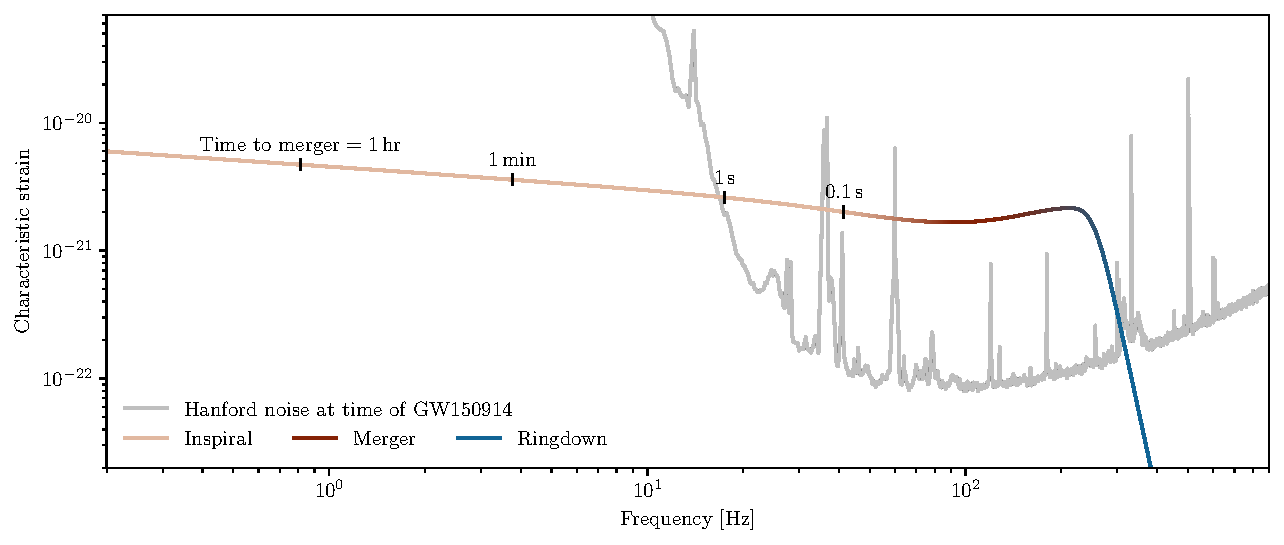
\includegraphics[width=\columnwidth]{Introduction/fd_waveform.pdf}
	\caption[The frequency-domain gravitational-wave signal from a binary black-hole merger]{ 
		The frequency-domain gravitational-wave signal from a binary black-hole merger, shown with the Hanford sensitivity curve (both expressed through the characteristic strain). The signal was generated with IMRPhenomD using parameters consistent with GW150914.}
	\label{fig:ch1:fd_waveform}
\end{figure}

The above discussion disregards the sensitivity of the detector to different frequencies (i.e.\ the detector noise).
It is standard to treat the noise in the LIGO and Virgo detectors as stationary and Gaussian~\cite{LIGOScientific:2019hgc}.
Stationarity means that the noise covariance matrix is diagonal in the frequency domain (meaning there is no correlation between frequency bins), and so we can describe the noise with a power spectral density (PSD) $S_n(f)$.
The noise in each frequency bin is modelled as following a Gaussian distribution with a random phase and amplitude $\sqrt{S_n(f)}$.
We show the Hanford PSD in Fig.~\ref{fig:ch1:fd_waveform}, along with a frequency-domain representation of a BBH GW signal. 
Since we are now comparing with a PSD, we fix the BBH total mass and distance to the example numbers used above ($M = 72\,M_\odot$, $r = 440\,\mathrm{Mpc}$).
Roughly speaking, the GW signal from a BBH merger increases in frequency over time.
The majority of the inspiral signal is at too low a frequency to be detected, with the GW signal only entering the detector band ($\sim 20$ to $\sim 1000\,\mathrm{Hz}$) just before merger.
Although the binary can spend millions of years inspiralling, we observe only the last few tenths of a second of the merger.
We choose to plot the signal and noise curve in terms of the characteristic strain~\cite{Moore:2014lga}, given by
\begin{equation}
    h_c(f) = 2f\abs{\tilde{h}(f)}
\end{equation}
for the GW signal (where $\tilde{h}$ is the frequency-domain GW in a given detector), and
\begin{equation}
    h_n(f) = \sqrt{fS_n(f)}
\end{equation}
for the noise curve.
The characteristic strain has the property that the area between the signal and noise curve is related to the signal-to-noise ratio (SNR) $\rho$ via
\begin{equation}
    \rho^2 = \int_{-\infty}^\infty \dd\log{f} \qty[\frac{h_c(f)}{h_n(f)}]^2.
\end{equation}
Evaluating for the above figure we get $\rho \sim 17$, which is consistent with the Hanford SNR for GW150914.

Also shown in the figure is the time to merger at select frequencies of the inspiral.
This is to emphasise how the frequency of the binary evolves over time, spending the vast majority of its life in the inspiral with a slowly shrinking orbit.
The time to merger, $\tau_\mathrm{merge}$, as a function of GW frequency is given by
\begin{equation}\label{eq:time_to_merger}
    \tau_\mathrm{merge} = \frac{5}{256} \qty(\pi f)^{-\frac{8}{3}} \qty(\frac{G\mathcal{M}}{c^3})^{-\frac{5}{3}},
\end{equation}
where $\mathcal{M}$ is a combination of the two masses in the binary known as the chirp mass.
We also explicitly show the factors of $G$ and $c$ in this equation for clarity (in geometric units these would be set to 1, and it would be implied that the chirp mass should be expressed in units of time). 
\comment{This expression comes from equating the time derivative of the orbital energy... worth showing?}

The signal in Fig.~\ref{fig:ch1:fd_waveform} was generated with the IMRPhenomD~\cite{Khan:2015jqa} waveform model, as implemented in the \texttt{ripple}~\cite{Edwards:2023sak} Python package.
Phenom models produce approximate waveforms using closed-form analytic expressions in the frequency-domain, making evaluation quick and suitable for GW searches.
The Hanford PSD is estimated from $1024\,\mathrm{s}$ of off-source data at the time of GW150914, using a Welch periodogram~\cite{1161901}.


\section{Black-hole ringdown}

The endpoint of a BBH, the ringdown signal is produced by the remnant BH settling to its stationary state.
Just as a bell or drum has a characteristic sound, so too does a BH; associated with the BH is a unique spectrum of oscillatory modes, determined purely by its properties (namely, for astrophysical BHs, a mass and spin).
The characteristic oscillations of the remnant BH are called quasinormal modes (QNMs), so-called because, unlike normal modes, they decay over time~\cite{Berti:2005ys, Berti:2009kk}.
The QNM frequencies are complex, $\omega = 2\pi f - i/\tau$, with the real part $f$ giving the oscillation frequency and the reciprocal of the imaginary part $\tau$ giving the damping time. 
The QNM spectrum is the subject of Section~\ref{ch1:sec:qnms}.
The ringdown signal consists of a sum of QNMs, each excited a different amount depending on the initial configuration of the binary and how they merged; the excitation of different ringdown modes is among the areas of investigation in Chapter.~\ref{Chapter2}.

\begin{figure}[ht!]
	\centering
	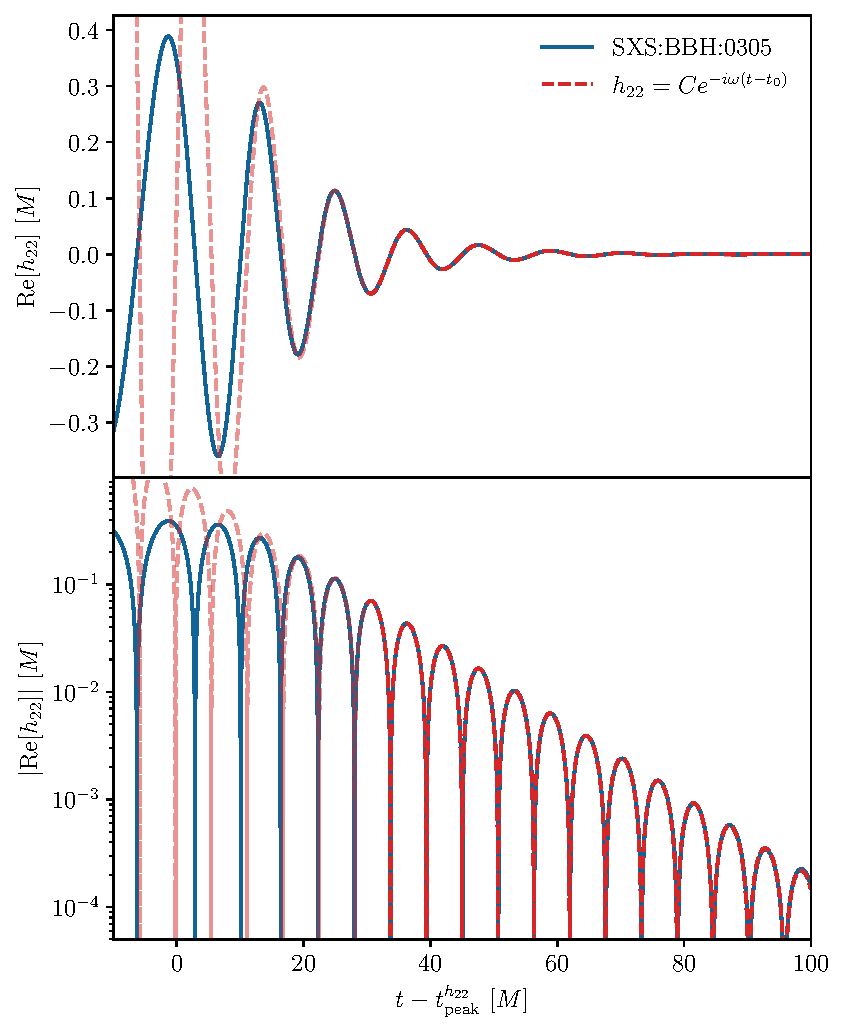
\includegraphics[width=\columnwidth]{Introduction/ringdown_waveform.pdf}
	\caption[The gravitational-wave ringdown signal]{ 
		The ringdown waveform from a BBH, fitted with a simple damped sinusoid. At early times this simple description breaks down. The waveform is a NR simulation from the SXS catalog.}
	\label{fig:ch1:rd_waveform}
\end{figure}

Fig.~\ref{fig:ch1:rd_waveform} shows (in blue) the ringdown waveform from a NR simulation, SXS:BBH:0305~\cite{Lovelace:2016uwp}.
This simulation has properties consistent with GW150914, and will be among the NR simulations studied in Chapter~\ref{Chapter2}.
NR waveforms are decomposed into spherical-harmonic modes indexed by $\ell$ and $m$ \comment{(see Section... for more details)}, and here we plot the real part of the dominant $\ell = m = 2$ mode.
The radial dependence of GW waveforms goes predominantly as $r^{-1}$, so the SXS catalog provides the strain multiplied by $r$ (just as what was plotted in Fig.~\ref{fig:ch1:td_waveform}).
For clarity we will drop the $r$ factor for the remainder of the thesis and have the $r^{-1}$ scaling implied (just keep in mind when we refer to the GW signal $h$ or a mode $h_{\ell m}$, we really mean $rh$ and $rh_{\ell m}$). 

Overplotted is a simple model for the $h_{22}$ mode: a exponentially damped sinusoid with complex frequency $\omega = 2\pi f - i/\tau$ and amplitude $C = Ae^{i\phi}$. 
Taking the real part we have
\begin{align}
    \Re[Ce^{-i\omega(t-t_0)}] &= \Re[Ae^{i\phi}e^{-i(2\pi f - i/\tau)(t-t_0)}] \nonumber \\
    &= \Re[Ae^{-i\qty[2\pi f(t-t_0) - \phi]}e^{-(t-t_0)/\tau}] \nonumber \\
    &= A\cos[2\pi f(t-t_0) - \phi]e^{-(t-t_0)/\tau}.
\end{align}
That such a simple model describes the final stages of such a complicated system is a remarkable result, and is part of the power of studying the ringdown.
A faded red line traces the damped sinusoid to earlier times, where it starts to lose validity.
This is to be expected: at earlier times we approach the nonlinear and strong-gravity merger, where BH perturbation theory (which is where this linear description comes from) starts to break down.
Note, however, that our model here only includes a single term (i.e., one ringdown QNM); with additional QNMs we may be able to get a better fit to the NR waveform, or to describe the waveform at earlier times (this idea is explored at length in Chapter~\ref{Chapter2}).
A particular subset of QNMs, known as ``overtones'', will be of particular interest throughout the thesis; as well as featuring in the numerical studies of Chapter~\ref{Chapter2}, they will be a target in the analysis of GW data in Chapters~\ref{Chapter3} and \ref{Chapter4}.

A key goal in GW astronomy is the identification of QNMs in the ringdown signal.
The testing GR companion papers for the second~\cite{LIGOScientific:2020tif} and third~\cite{LIGOScientific:2021sio} GW event catalogs featured searches for QNMs; of the detected events, results were reported for 22.
This can be taken as a rough guide for how many events have at least one measurable ringdown mode.
On top of this, tentative evidence was reported for the identification of an additional ringdown mode in a few of the loudest events, including GW150914.
However, as will be seen, the identification of subdominant ringdown modes is subtle.
This is particularly true for one of the most massive BBH mergers observed so far, GW190521~\cite{LIGOScientific:2020iuh}, which has a total source frame mass of $\sim 150\,M_\odot$.
Its large mass means this event enters the detector band only very near merger, and so is ringdown dominated.
This makes it a promising target for QNM searches, and along with GW150914 it is an event that will be referenced throughout this thesis. 

% GWTC-2: GW150914 and GW190521_074359 show some signs of an overtone. Mention contention re overtone? Probably best to save for later. 
% An event on the same day, known just as GW190521 CITE, is of particular interest to ringdown studies because of its exceptionally high mass. Not much inspiral... ringdown dominated... and analyses by others have claimed the identification of a higher harmonic.
% GWTC-3: GW200224_222234 shows log10B ~ 0.95 evidence for overtone

% If a system has a set of characteristic frequencies associated with it, then if we excite the system we can attempt to measure those frequencies and characterise the system. This is spectroscopy...

\section{Quasinormal modes}
\label{ch1:sec:qnms}

\comment{
The QNM frequencies can be calculated within the framework of linearised gravity, treating the gravitational field in the vicinity of the remnant as a small (linear) perturbation of the Kerr metric \cite{Berti:2009kk}.
Therefore, the QNM description of the GW signal is only expected to be valid at sufficiently late times, when the nonlinearities from the merger have largely decayed away. 
}

\comment{
\begin{itemize}
    \item Polar (even-parity) Schwarzschild metric perturbations are described by the Zerilli equation \cite{Zerilli:1970se, Zerilli:1970wzz}, and axial (odd-parity) perturbations are described by the Regge-Wheeler equation \cite{Regge:1957td} (interestingly, these two equations are isospectral, with identical QNM spectra).
    \item Teukolsky obtains separable wave equations for electromganetic and gravitational perturbations of a rotating BH~\cite{Teukolsky:1972my}.
\end{itemize}
}

\comment{
The remnant Kerr BH has no hair; it is fully described by only a final mass and a dimensionless final spin parameter. 
The same is true of the spectrum of QNM frequencies, which are also functions of only the mass and spin. 
This offers the opportunity for some clean tests of GR... discussed further in Section~\ref{ch1:sec:bh_spectroscopy}.
}

\comment{
QNMs also have practical uses in waveform modelling. They are used in full inspiral-merger-ringdown BBH waveforms produced in both the phenomenological \cite{Pratten:2020ceb, Garcia-Quiros:2020qpx, Pratten:2020fqn} and effective-one-body approaches \cite{Buonanno:2006ui, Buonanno:2007pf, Pan:2011gk}.
}

\subsection{Scalar field on a Schwarzschild background}

To help build some intuition regarding the origin of the QNMs, we will perform a demonstrative calculation involving a massless scalar field, $\psi(t,r,\theta,\phi)$ on a Schwarzschild background.
This will lead to equations reminiscent of the Zerilli and Regge-Wheeler equations, without the complication of tensor spherical harmonics that comes with the full gravitational-perturbation treatment.
The metric tensor, in Schwarzschild coordinates, is
\begin{equation}
g_{\mu\nu} = \begin{pmatrix}
- \left(1 - \frac{2M}{r}\right) & 0 & 0 & 0 \\
0 & \left(1 - \frac{2M}{r}\right)^{-1} & 0 & 0 \\
0 & 0 & r^2 & 0 \\
0 & 0 & 0 & r^2 \sin^2\theta
\end{pmatrix},
\end{equation}
where now $M$ is the mass of the BH (and not the total mass of the binary, as before). 
The scalar field evolves according to the Klein-Gordon equation 
\begin{equation}
    \nabla_\mu \nabla^\mu \psi = 0.
\end{equation}
Using the fact that a covariant derivative reduces to the partial derivative on scalars, we can write this as
\begin{equation}
    \nabla_\mu \nabla^\mu \psi = \frac{1}{\sqrt{-g}} \partial_\mu \qty(\sqrt{-g} g^{\mu\nu} \partial_\nu \psi) = 0
\end{equation}
where $g$ is the determinant of the metric tensor, $g^{\mu\nu}$ is the inverse of the metric tensor, and we have also used $\Gamma^\mu_{\mu\nu} = \partial_\nu \ln{\sqrt{-g}} = \qty(-g)^{-1/2} \partial_\nu \sqrt{-g}$.
For Schwarzschild we have $g = -r^4 \sin^2{\theta} \implies \sqrt{-g} = r^2 \sin{\theta}$.
Evaluating, we get
\begin{multline}
    - \qty(1 - \frac{2M}{r})^{-1} \pdv[2]{\psi}{t} + \frac{1}{r^2} \pdv{r} \qty[r^2 \qty(1 - \frac{2M}{r}) \pdv{\psi}{r} ]\\
    + \frac{1}{r^2} \qty[ \frac{1}{\sin{\theta}} \pdv{\theta} \qty(\sin{\theta} \pdv{\psi}{\theta} ) + \frac{1}{\sin^2{\theta}} \pdv[2]{\psi}{\phi} ] = 0.
\end{multline}
Recognising that the spherical harmonics, $Y_{\ell m}(\theta,\phi)$, are the eigenfunctions of the angular part:
\begin{equation}
    \frac{1}{\sin{\theta}} \pdv{\theta} \qty(\sin{\theta} \pdv{Y_{\ell m}}{\theta} ) + \frac{1}{\sin^2{\theta}} \pdv[2]{Y_{\ell m}}{\phi} = - \ell (\ell + 1) Y_{\ell m},
\end{equation}
we will attempt a spherical harmonic decomposition of the scalar field. 
With the expectation that the radial dependence of the field will go as $1/r$ (and also anticipating a change in radial coordinate) we write the scalar field as
\begin{equation}
    \psi(t, r, \theta, \phi) = \frac{1}{r} \sum_{\ell = 0}^\infty \sum_{m = -\ell}^\ell \psi_{\ell m}(t, r) Y_{\ell m}(\theta, \phi).
\end{equation}
Note that here, in the scalar case, the sum over $\ell$ starts from $\ell = 0$.
In general, the sum will start from $\ell = \abs{s}$, where $s$ is the spin weight of the field ($s=0$, $-1$ and $-2$ for scalar, electrical, and gravitational perturbations respectively).
Substituting, we are left with an equation for the radial part:
\begin{multline}
    - \pdv[2]{\psi_{\ell m}}{t} + \frac{1}{r} \qty(1 - \frac{2M}{r}) \pdv{r} \qty[r^2 \qty(1 - \frac{2M}{r}) \pdv{r}\qty(\frac{\psi_{\ell m}}{r}) ]\\
    - \qty(1 - \frac{2M}{r}) \qty(\frac{\ell (\ell + 1)}{r^2}) \psi_{\ell m} = 0.
\end{multline}
To proceed we introduce the tortoise coordinate, $r_*$,
\begin{equation}
    r_* = r + 2M \ln(\frac{r}{2M} - 1),
\end{equation}
which has the property that
\begin{equation}
    \dv{r_*}{r} = \qty( 1 - \frac{2M}{r} )^{-1}.
\end{equation}
Note that as $r$ approaches the Schwarzschild radius ($r \rightarrow 2M$), the tortoise coordinate $r_* \rightarrow -\infty$.
Making this change of variables, we arrive at
\begin{equation}\label{eq:wave_equation}
    \pdv[2]{\psi_{\ell m}(t,r)}{r_*} - \pdv[2]{\psi_{\ell m}(t,r)}{t} - V_\ell(r) \psi_{\ell m}(t,r) = 0,
\end{equation}
where
\begin{equation}
    V_\ell(r) = \qty( 1 - \frac{2M}{r} ) \qty( \frac{\ell (\ell + 1)}{r^2} + \frac{2M}{r^3} )
\end{equation}
is an effective potential.
Performing a Fourier transform, we can bring Eq.~\ref{eq:wave_equation} into the form of a one-dimensional Schr\"{o}dinger equation
\begin{equation}\label{eq:fd_wave_equation}
    \pdv[2]{\tilde{\psi}_{\ell m}(\omega,r)}{r_*} + \qty[ \omega^2 - V_\ell(r)] \tilde{\psi}_{\ell m}(\omega,r) = 0.
\end{equation}
Axial gravitational perturbations obey an equation of the same form (i.e. the Regge-Wheeler equation), and in fact the effective potential can be written in the unified form
\begin{equation}
    V_\ell(r) = \qty( 1 - \frac{2M}{r} ) \qty( \frac{\ell (\ell + 1)}{r^2} + \frac{(1 - s^2)2M}{r^3} )
\end{equation}
with $s = 0$, $-1$ and $-2$ for scalar, electrical, and gravitational perturbations respectively. 
The Zerilli equation, describing polar perturbations, also has a similar form (but with a more complicated effective potential). 
Regardless, it has been shown that the Regge-Wheeler and Zerilli equations give the same QNM spectrum \cite{Chandrasekhar:1975nkd}.

\begin{figure}[t]
    \centering
    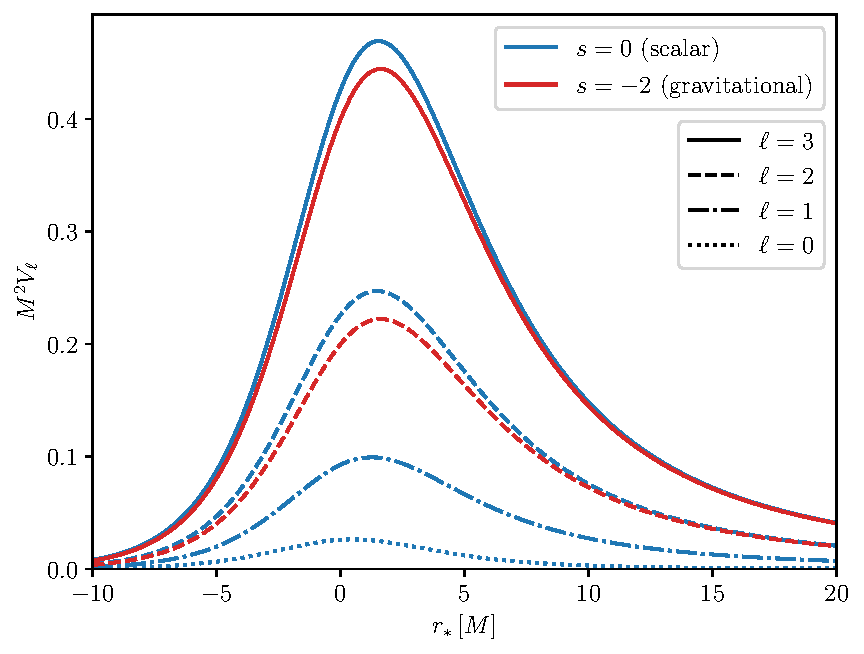
\includegraphics[width=0.8\columnwidth]{Figures/Introduction/rw_potential.pdf}
    \caption[The Regge-Wheeler potential]{The Regge-Wheeler potential as a function of the tortoise coordinate $r_*$ (with the BH horizon at $r_* = -\infty$), for scalar and gravitational perturbations and for a selection of $\ell$. In this subsection $M$ refers to the mass of the Schwarzschild BH, and not the total binary mass.}
    \label{fig:rw_potential}
\end{figure}

We must specify boundary conditions to complete the problem. 
When solving for the normal modes on a string, or the energy levels of a quantum harmonic oscillator, we require the wavefunction to vanish at the boundaries (either at the string ends, or at $\pm \infty$ for the harmonic oscillator).
The problem we're considering here is slightly different; the potential, depicted in Fig.~\ref{fig:rw_potential}, clearly does not admit bound states. 
Instead, the potential vanishes for $r_* \rightarrow \pm \infty$, which implies we need to look for purely outgoing plane waves:
\begin{alignat}{2}
    &\tilde{\psi}_{\ell m}(\omega, r) \sim e^{i \omega r_*} \qquad &&\qty(r_* \rightarrow -\infty) \nonumber \\
    &\tilde{\psi}_{\ell m}(\omega, r) \sim e^{- i \omega r_*} \qquad &&\qty(r_* \rightarrow \infty).
\end{alignat}
This follows from the consideration that the field should radiate  only inward at the horizon and only outward at spatial infinity.
When enforcing these boundary conditions, only discrete values of $\omega$ satisfy Eq.~\ref{eq:fd_wave_equation}; these are the QNMs.
In the case of a Kerr BH, we denote the QNMs $\omega_{\ell m n}$.
They are indexed by three numbers: the usual angular indices $\ell$ and $m$, and an additional ``overtone'' index $n$.

Several methods have been employed to calculate QNMs, including shooting methods \cite{Chandrasekhar:1975zza}, WKB methods \cite{Schutz:1985km}, and continued fractions \cite{Leaver:1985ax}.
The latter is known to be highly accurate, and is the method of choice in modern codes such as the \texttt{qnm} Python package \cite{Stein:2019mop} (which is used throughout this thesis).

\comment{Cite the vibrating string paper somewhere here?~\cite{Berti:2006wq}}

\subsection{Quasinormal modes from the geodesic correspondence}

First pointed out by Goebel~\cite{1972ApJ...172L..95G}, there exists a relation between BH QNMs and null geodesics around the BH spacetime.
Having since been developed further~\cite{Ferrari:1984zz, Mashhoon:1985cya, Cardoso:2008bp, Yang:2012he}, this approach provides a physical insight to QNMs; that is, QNMs can be interpreted as GWs slowly leaking out of a light-ring orbit around the BH. 
Although only valid for $\ell \gg 1$ (known as the eikonal, or geometrical optics, limit), this correspondence greatly simplifies the calculations of QNMs since it only depends on the background metric.
Consequently, it offers a way to compute QNMs in beyond GR theories (for example, as was done in Ref.~\cite{Blazquez-Salcedo:2016enn}), or for computing the QNM spectrum for charged (Kerr-Newman~\cite{Newman:1965my}) BHs~\cite{Cardoso:2016olt, Wang:2021uuh} (but, see also Ref.~\cite{Carullo:2021oxn} where a more sophisticated analysis was done).

The key result is that the QNM frequencies for a Kerr BH in the eikonal limit can be written as
\begin{equation}
    \omega_{\ell m n} = \qty(\ell + \frac{1}{2}) \Omega_\theta + m \Omega_\mathrm{pre} - i \qty(n + \frac{1}{2}) \gamma_L.
\end{equation}
Here, $\Omega_\theta$ is the frequency of small geodesic oscillations in the polar direction. 
The precessional frequency of the orbital plane, $\Omega_\mathrm{pre}$, is given by $\Omega_\mathrm{pre} = \Omega_\phi - \Omega_\theta$, where $\Omega_\phi$ is the orbital frequency of the light ring.
Finally, $\gamma_L$ is the Lyapunov exponent of the light ring; this can be thought of as a measure of the stability of the orbit.
Crucially, these quantities are all determined by the metric. 
Below we take a simple case of an axisymmetric spacetime and show how one can calculate the relevant quantities.
As a further simplification we also focus on the $\ell = m$ case, since these modes are associated with equatorial motion. 
Note that, with the assumption $\ell = m \gg 1$, we can write the real part of the QNM frequency as
\begin{equation}
    \qty(\ell + \frac{1}{2}) \Omega_\theta + m \Omega_\mathrm{pre} \sim \ell \Omega_\theta + \ell \qty(\Omega_\phi - \Omega_\theta) = \ell \Omega_\phi,
\end{equation}
which aligns with the interpretation of QNMs originating as GWs in light ring orbits.

First, we need the metric associated with a stationary and axisymmetric spacetime. 
The stationary and axisymmetric character requires that the metric coefficients be independent of $t$ and $\phi$, so that $g_{\mu \nu} = g_{\mu \nu}(r,\theta)$.
We also require that the spacetime is invariant to the simultaneous inversion of the time $t$ and the angle $\phi$ (i.e.\ to the transformation $t \rightarrow -t$, $\phi \rightarrow -\phi$). 
The physical meaning is that the spacetime we are considering is that associated with a rotating body. 
This invariance requires 
\begin{equation}
	g_{tr} = g_{t \theta} = g_{\phi r} = g_{\phi \theta} = 0.
\end{equation}
Then we have 
\begin{equation}
	\dd s^2 = g_{tt}\dd t^2 + 2g_{t \phi} \dd t \dd \phi + g_{\phi \phi}\dd \phi^2 + \qty[ g_{rr}\dd r^2 + 2g_{r \theta} \dd r \dd \theta + g_{\theta \theta} \dd \theta^2 ].
\end{equation}
It can be shown \cite{Chandrasekhar:1985kt} that the term in square brackets can be brought to the diagonal form $g_{r'r'}\dd r'^2 +  g_{\theta' \theta'} \dd \theta'^2$ by a change of coordinates $r'=r'(r,\theta)$ and $\theta'=\theta'(r,\theta)$.
Renaming our variables by removing the primes, this gives
\begin{equation}
	\dd s^2 = g_{tt}\dd t^2 + g_{rr}\dd r^2 + g_{\theta \theta}\dd \theta^2 + g_{\phi \phi}\dd \phi^2 + 2g_{t \phi}\dd t\dd \phi
\end{equation}
We can find geodesic curves $x^\mu(\lambda)$ by extremising the action $S=\int\mathrm{d}\lambda\,\mathcal{L}$ where the Lagrangian is given by
\begin{align}
	\mathcal{L} &= \frac{1}{2}g_{\mu \nu} \dot{x}^\mu \dot{x}^\nu \\
	&= \frac{1}{2}\qty(g_{tt}\dot{t}^2 + g_{rr}\dot{r}^2 + g_{\theta \theta}\dot{\theta}^2 + g_{\phi \phi}\dot{\phi}^2 + 2g_{t \phi}\dot{t}\dot{\phi}), \nonumber
\end{align}
and a dot denotes a derivative with respect to the affine parameter $\lambda$ along the curve. 
We could find the second order differential geodesic equations from the Euler-Lagrange (EL) equations, 
\begin{gather} \label{eq:ELeqns_1}
	\dv{\lambda}(\pdv{\mathcal{L}}{\dot{x}^\mu}) = \pdv{\mathcal{L}}{x^\mu}.
\end{gather}
However, first we recognise that the spacetime, and hence the action, are stationary; therefore the timelike component of the 4-momentum is a constant of the motion
\begin{equation}\label{eq:el_t} 
	\pdv{\mathcal{L}}{\dot{t}} = -E \;\implies\; g_{tt}\dot{t} + g_{t\phi}\dot{\phi} = -E.
\end{equation}
Similarly, from the axisymmetry of the spacetime we have another constant of motion $L$,
\begin{equation}\label{eq:el_phi}
	\pdv{\mathcal{L}}{\dot{\phi}} =L \;\implies\; g_{\phi \phi}\dot{\phi} + g_{t\phi}\dot{t} = L.
\end{equation}
From Eqs.~\ref{eq:el_t} and \ref{eq:el_phi} we can solve for the two components of the 4-velocity $\dot{t}$ and $\dot{\phi}$ to give
\begin{gather} \label{eq:tdot_L}
	\dot{t} = E \frac{g_{\phi \phi} + g_{t \phi}\hat{L}}{\qty(g_{t \phi})^2 - g_{t t}g_{\phi \phi}} \\
	\label{eq:phidot_L}
	\dot{\phi} = E \frac{g_{t \phi} + g_{t t}\hat{L}}{g_{t t}g_{\phi \phi} - \qty(g_{t \phi})^2}
\end{gather}
where $\hat{L} = L/E$.
We are also free to rescale our affine parameter $\lambda\rightarrow E\lambda$ to remove $E$ from the above expressions.
The azimuthal orbital frequency can also be calculated:
\begin{gather}
	\Omega_\phi = \frac{\mathrm{d}\phi}{\mathrm{d}t} =  \frac{\dot{\phi}}{\dot{t}} = -\frac{g_{t\phi}+g_{tt}\hat{L}}{g_{\phi\phi}+g_{t\phi}\hat{L}}
\end{gather}
In general, for the remaining two coordinates, $r$ and $\theta$, we can use the EL equations to find the second order differential geodesic equations.
However, in the special case of equatorial motion ($\theta=\pi/2\;\implies\;\dot{\theta}=0$) we can get a first order equation for $\dot{r}$ by considering the normalization of the four-velocity;
\begin{equation} \label{eq:rdot}
	g_{\mu\nu}\dot{x}^\mu\dot{x}^\mu = 0 \;\implies\; \dot{r}^2 = V_{\rm eff}(r;\hat{L}),
\end{equation}
where
\begin{align}\label{eq:Veff}
	V_{\rm eff}(r;\hat{L}) &= \frac{-g_{tt}\dot{t}^2 -g_{\phi\phi}\dot{\phi}^2-2g_{t\phi}\dot{t}\dot{\phi} }{g_{rr}} \nonumber \\
	&= \frac{g_{tt} \hat{L}^2+2 g_{t\phi } \hat{L}+g_{\phi\phi}}{g_{rr}(g_{t\phi}^2-g_{tt} g_{\phi \phi})},
\end{align}
and in the final line we have used Eqs.~\ref{eq:tdot_L} and \ref{eq:phidot_L} to eliminate $\dot{t}$ and $\dot{\phi}$.
In Eq.~\ref{eq:Veff} it is to be understood that the $g_{\mu\nu}$ metric coefficients are to be evaluated on the equatorial plane $\theta=\pi/2$ and so are only functions of $r$.

A light ring is circular null geodesic orbit. 
The radius, $r_*$, and angular momentum, $\hat{L}_*$, of such an orbit must satisfy $V_{\rm eff} = V'_{\rm eff} = 0$, where a prime denotes a radial derivative with respect to $r$. The first condition yields
\begin{equation}
	\hat{L}_*(r) = \frac{-g_{t \phi} \pm \sqrt{g_{t \phi}^2 - g_{t t}g_{\phi \phi}}}{g_{t t}},
\end{equation}
while the second gives an implicit formula for $r_*$:
\begin{gather}
	V'_{\rm eff}\big(r_*;\hat{L}_*(r_*)\big) = 0.
\end{gather}
% In the case of the Kerr metric single root $r_*$.

Having found the equations of the light ring, now consider neighbouring geodesics. 
First, consider polar motion. The EL for $\theta$ (Eq.~\ref{eq:ELeqns_1} with $x^\mu=\theta$) is 
\begin{multline}\label{eq:el_theta}
	g_{\theta \theta} \ddot{\theta} + \qty(\pdv{g_{\theta \theta}}{\theta} \dot{\theta} + \pdv{g_{\theta \theta}}{r} \dot{r}) \dot{\theta} \\
	= \frac{1}{2} \bigg(\pdv{g_{t t}}{\theta} \dot{t}^2 + \pdv{g_{r r}}{\theta} \dot{r}^2 + \pdv{g_{\theta \theta}}{\theta} \dot{\theta}^2 + \pdv{g_{\phi \phi}}{\theta} \dot{\phi}^2 + 2\pdv{g_{t \phi}}{\theta} \dot{t}\dot{\phi}\bigg).
\end{multline}
Consider small perturbations in the $\theta$ direction about the light ring; i.e. set $r = r_*$, $\theta = \pi/2+\delta\theta(\lambda)$, and where $\dot{t}$ and $\dot{\phi}$ are given by Eqs.~\ref{eq:tdot_L} and \ref{eq:phidot_L} respectively and discard terms $\mathcal{O}(\delta\theta^2)$. 
This gives
\begin{multline}\label{eq:el_theta_expanded}
	g_{\theta \theta}(r_*,\pi/2) \ddot{\delta \theta} \\
 = \frac{1}{2} \bigg(\pdv[2]{g_{t t}(r_*,\pi/2)}{\theta} \dot{t}^2 + \pdv[2]{g_{\phi\phi}(r_*,\pi/2)}{\theta} \dot{\phi}^2 + 2\pdv[2]{g_{t \phi}(r_*,\pi/2)}{\theta} \dot{t}\dot{\phi}\bigg)\delta \theta.
\end{multline}
which describes simple harmonic motion, $\ddot{\delta\theta}=-\tilde{\Omega}^2_\theta\delta\theta$, where the constant $\tilde{\Omega}_\theta$ is the frequency of the oscillations with respect to the parameter $\lambda$.
The frequency of the oscillations with respect to coordinate time $t$ is given by
\begin{align}
	\Omega_\theta = \frac{\tilde{\Omega}_\theta}{\dot{t}} =\sqrt{-\frac{
			\pdv[2]{g_{t t}}{\theta} +2\pdv[2]{g_{t \phi}}{\theta} \Omega_\phi + \pdv[2]{g_{\phi\phi}}{\theta} \Omega_\phi^2
		}{2g_{\theta \theta}}} ,
\end{align}
where all quantities on the right hand side are to be evaluated at the light ring. 
In the case of the Kerr metric $\Omega_\theta^2>0$ and the light ring is stable in the polar direction.

Now consider motion in the radial direction ($\dot{r}\neq 0$).
Differentiating Eq.~\ref{eq:rdot} with respect to $\lambda$ gives
\begin{align}
	\ddot{r} = \frac{1}{2}V'_{\rm eff}(r).
\end{align}
Consider small perturbations $r = r_*+\delta r(\lambda)$ with $\theta = \pi/2$ and discarding $\mathcal{O}(\delta r^2)$ terms gives
\begin{align}
	\ddot{\delta r} = \frac{1}{2}V''_{\rm eff}(r_*)\delta r.
\end{align}
Looking for periodic solutions, the frequency of the radial oscillaitons (with respect to coordinate time) is given by
\begin{align}
	\Omega_{r} = \sqrt{-\frac{V''_{\rm eff}(r_*)}{2\dot{t}^2}}.
\end{align}
In the case of the Kerr metric the light ring orbit has $\Omega_r^2<0$ and is unstable in the radial direction; therefore $\gamma_L = (-\Omega_r^2)^{-1/2}$ is the instability (Lyapunov) timescale.

\section{Black-hole spectroscopy}
\label{ch1:sec:bh_spectroscopy}

The full Kerr QNM spectrum is nowadays readily available, with modern codes (such as the \texttt{qnm} package~\cite{Stein:2019mop}) making use of a version of Leaver's method~\cite{Leaver:1985ax} to compute them.
We show the $\ell = 2$, $n = 0$; $\ell = 3$, $n = 0$; and $\ell = 2$, $n = 1$ branches of the spectrum in Fig.~\ref{fig:ch1:qnm_taxonomy} (of course, the full spectrum would extend to infinity in both $\ell$ and $n$, but the branches shown here include the QNMs of most interest at current detector sensitivities).  
\comment{
Usually, the GW strain is dominated by the $\ell=|m|=2$ modes. 
Furthermore, the overtones decay more quickly (i.e.\ $\tau$ decreases) with increasing $n$ so that at late times the signal will be dominated by the fundamental $n=0$ modes. 
Therefore, the most prominent QNM in the ringdown is expected to be the $(\ell, m, n)=(2,2,0)$ mode, and the observational challenge is usually to detect the presence of other, subdominant modes.
}
There are different conventions used in the literature to label the modes; we aim to clarify these with Fig.~\ref{fig:ch1:qnm_taxonomy}.
Firstly, we see the QNMs appear to come in pairs: those with positive real part, and those with negative real part.
These are the ``regular'' and ``mirror'' (sometimes called ``twin'' or ``conjugate'') QNMs respectively.
Denoting the mirror QNM frequency with a prime, we can relate $\omega'_{\ell m n}$ to the regular QNMs as follows~\cite{Berti:2005ys}:
\begin{equation}
    f'_{\ell m n} = -f_{\ell -m n}, \quad \tau'_{\ell m n} = \tau_{\ell -m n} \nonumber
\end{equation}
\begin{equation} 
    \quad\Rightarrow\quad \omega'_{\ell m n} = - \omega_{\ell -mn}^*.
    \label{ch1:eq:mirror}
\end{equation}
So, for example, when we refer to the ``$(2,-2,0)$ mirror mode'', we are referring to the mode which has a real (imaginary) part negative (the same as) the regular $(2,2,0)$ mode.
This way of referring to the modes allows us to unambiguously refer to every mode in the spectrum, including the $m=0$ modes, and will be the preferred method in this work.

\begin{figure}[t]
	\centering
	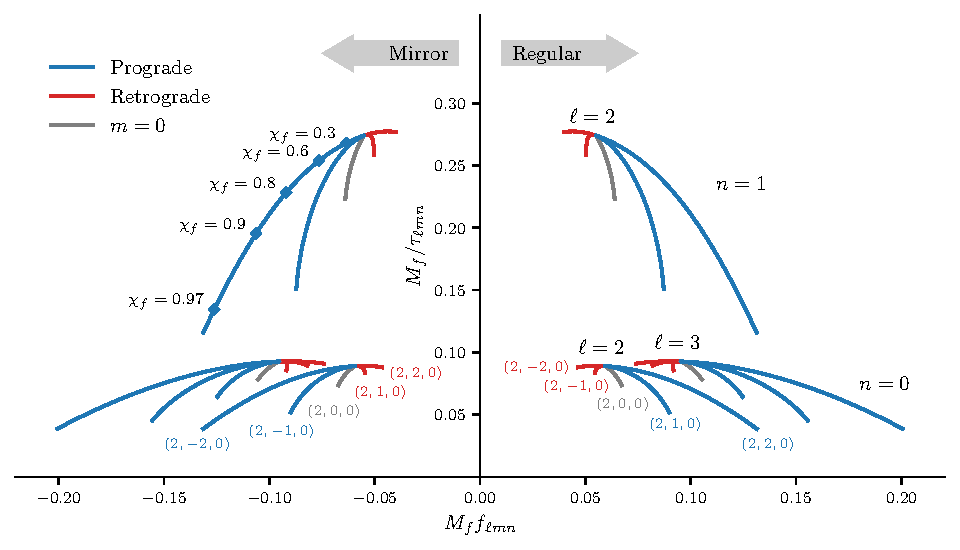
\includegraphics[width=\columnwidth]{Introduction/qnm_taxonomy.pdf}
	\caption[The Kerr quasinormal mode spectrum]{ 
		Selected modes of the Kerr QNM spectrum. BH QNMs frequencies are conventionally represented as complex numbers, with the real part giving the  angular frequency of the mode and the imaginary part giving (minus) the inverse of the damping time: $\omega_{\ell m n} = 2\pi f_{\ell m n} - i/\tau_{\ell m n}$. Here we plot $f_{\ell m n}$ and $1/\tau_{\ell m n}$, each scaled by the remnant BH mass $M_f$ to make a dimensionless quantity. The spectrum of a Kerr BH also depends on the dimensionless BH spin magnitude, $\chi_f$; as the spin is increased from zero, branches with different $m$ appear and spread out from the points of the Schwarzschild spectrum.
        }
	\label{fig:ch1:qnm_taxonomy}
\end{figure}

We can, alternatively, split the spectrum into ``prograde'' and ``retrograde'' modes. 
This description has the advantage of having a clear physical interpretation; prograde (retrograde) modes are those that are corotating (counterrotating) with the final BH spin.
This can also be expressed as prograde modes satisfying $\mathrm{sgn}\qty(\Re[\omega_{\ell m n}]) = \mathrm{sgn}\qty(m)$, and retrograde modes satisfying $\mathrm{sgn}\qty(\Re[\omega_{\ell m n}]) = -\mathrm{sgn}\qty(m)$.
For binaries where the individual BHs have low spin (or aligned spins that rotate in the same sense as the orbit) it is also expected that the retrograde modes will be suppressed compared to the prograde modes, which is simply a result of the geometry of merger exciting prograde modes (this has also been shown by studies of numerical simulations, for example in Refs.~\cite{Berti:2005ys, London:2014cma, JimenezForteza:2020cve}).
This assumption is less clear for precessing systems, and is investigated in Chapter~\ref{Chapter2}.

As previously mentioned, the remnant Kerr BH is fully described by only a final mass and a dimensionless final spin.
We now denote these quantities $M_f$ and $\chi_f = \abs{\vb*{\chi}_f}$, where the $f$ denotes ``final'' to avoid confusion with the binary properties.
Consequently, the Kerr QNM spectrum is also a function of only the remnant mass and spin.
In Fig.~\ref{fig:ch1:qnm_taxonomy} we can see the mass enters as a scaling on the axes, and the spin gives the position along each branch (we show select spin values along the $(2,-2,1)$ mirror mode branch).
The Schwarzchild spectrum, which depends only on the BH mass and has no $m$ dependence, can be recovered by plotting points at the branch point of each $(\ell, n)$ group.
% No-hair... allows us to do tests, in analogy with atomic spectroscopy...
% possible no-hair cite: https://journals.aps.org/prl/abstract/10.1103/PhysRevLett.26.331
% p60 of https://arxiv.org/pdf/0905.2975.pdf
% p151 of https://arxiv.org/pdf/1501.07274.pdf
% opening of https://arxiv.org/pdf/1905.00869.pdf

\comment{
The study of QNMs has applications in both astro and fundamental physics. 
The highly constrained dependence of the QNM spectrum on only the remnant mass and spin means that, conversely, if a QNM frequency is measured, then the mass and spin of the final BH merger can be inferred. 
For high-mass systems, where only the ringdown signal is observable, this may be the only information available about the nature of the source \cite{Berti:2005ys, Baibhav:2020tma}. 
For lower-mass systems, measuring QNM frequencies allows us to estimate the remnant properties independently of the rest of the signal, and so consistency tests can be performed. 
For example, a test of the BH area theorem can be performed in this way \cite{Cabero:2017avf, Isi:2020tac}. 
A similar consistency test using full inspiral-merger-ringdown models and a sharp cut in the frequency (rather than time) domain was performed on GW150914 \cite{LIGOScientific:2016lio}. 
Each additional QNM that can be detected in the ringdown provides a separate estimate of the mass and spin of the remnant. 
Therefore, if multiple QNM frequencies can be identified, a ringdown-only consistency test on the expected Kerr-like nature of the remnant BH can be performed \cite{Dreyer:2003bv, Carullo:2019flw} (this is possible only if the $(\ell, m, n)$ of the modes are known). 
In these tests, deviations from the expected results may point to new physics beyond GR. 
}

 \begin{figure}[t]
    \centering
    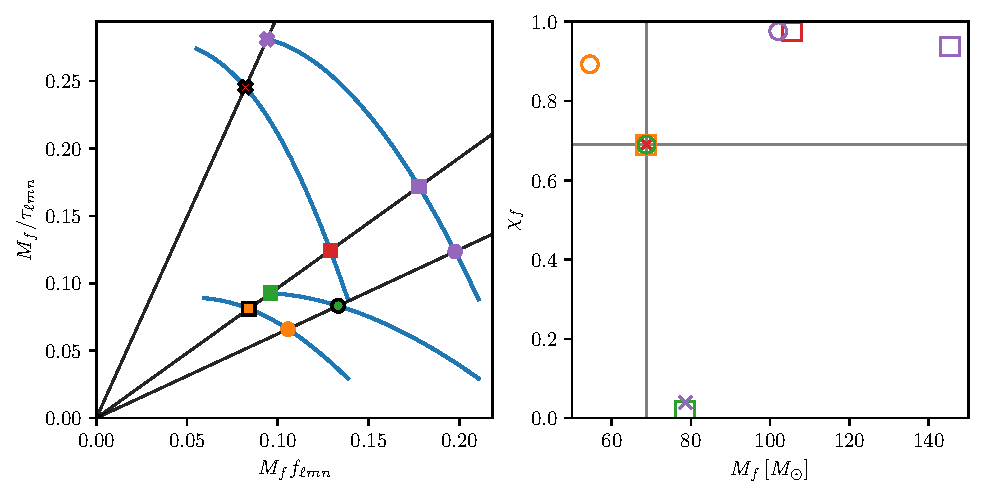
\includegraphics[width=\columnwidth]{Figures/Introduction/bh_spectroscopy.pdf}
    \caption[Black-hole spectroscopy illustration]{Black-hole spectroscopy: a frequency -- damping-time measurement corresponds to a straight line in the left panel. Three such measurements are shown, and their intersections with the Kerr spectrum are indicated. Each measurement is associated with a particular marker shape, and each Kerr branch is associated with a particular marker colour. Each intersection can be converted to a remnant BH mass and spin, shown on the right panel. Only one mass and spin is consistent with all three measurements; these are the true BH properties.}
    \label{fig:ch1:bh_spectroscopy}
\end{figure}

Fig.~\ref{fig:ch1:bh_spectroscopy} demonstrates the idea behind BH spectroscopy~\cite{Dreyer:2003bv}.
On the left panel we show four branches of the Kerr spectrum of Fig.~\ref{fig:ch1:qnm_taxonomy}; the (2,2,0), (2,2,1), (3,3,0) and (3,3,1) modes.
The (2,2,1) and (3,3,0) modes are promising targets for a QNM measurement beyond the fundamental mode, and currently they are the only modes for which there is possible evidence in GW observations~\cite{Isi:2019aib, Capano:2021etf} (these claims are, however, disputed).
In BH spectroscopy, we imagine directly measuring a frequency and damping time in the GW data; say, $f_*$ and $\tau_*$.
In the $M_f f_{\ell m n}$ -- $M_f/\tau_{\ell m n}$ space, this measurement corresponds to a straight line intersecting with the origin; this simply comes from the fact that our scale is not fixed, since we express everything in terms of $M_f$. 
Fixing the value of $M_f$ would collapse the line to a single point, $(f_*,\tau_*)$.
The gradient of the line is given by
\begin{equation}
    \frac{1}{f_* \tau_*} = \frac{\pi}{Q_*},
\end{equation}
where $Q_* = \pi f_* \tau_*$ is the quality factor of the measured mode.
We show three such measurements, and mark where they intersect the Kerr spectrum.
Each intersection corresponds to a particular remnant BH mass, $M_f$, and spin, $\chi_f$. 
The distance of the intersection along the Kerr branch gives the spin.
The mass is found by, for example, dividing the value of $M_f f_{\ell m n}$ at the intersection by the measured frequency $f_*$.
Since each measurement line intersects with multiple Kerr branches, they return multiple $(M_f, \chi_f)$ values. 
However, assuming the BH is indeed described by the Kerr metric, then there will be a single $(M_f,\chi_f)$ combination consistent with all the measurements (indicated by the horizontal and vertical lines in the right panel).
If no such combination exists, then what is observed is either not an isolated BH, or it is not described by Kerr.